\section{Equilibrium Points} \label{sec:EquilibriumPoints}

The equations of motion \eqref{eq:cr3bp_acceleration} derived in \cref{sec:CR3BP} can be reformulated in terms of the gradients of scalar fields, or \emph{potentials}. In particular, the inertial $(d^2\boldsymbol{r}/dt^2)_I$ and centrifugal $\boldsymbol{\omega} \times \left(\boldsymbol{\omega} \times \boldsymbol{r}\right)$ terms in \eqref{eq:inertial_transport_theorem}---the two conservative terms---are associated with a gravitational and centrifugal potential, respectively. Denoting the former as $U_g$ and the latter as $U_c$, these potentials are expressed as
\begin{align*}
    U_g &= -\frac{1-\mu}{\rho_1} - \frac{\mu}{\rho_2}, \\
    U_c &= -\frac{1}{2}\left(\boldsymbol{\omega} \times \boldsymbol{r}\right)\cdot\left(\boldsymbol{\omega} \times \boldsymbol{r}\right)
    = -\frac{1}{2}\left(x^2 + y^2\right).
\end{align*}
Combining the two yields the \emph{effective potential}, $\tilde{U} \coloneq U_g + U_c$. These potentials are visualized in \cref{fig:effective_potential}.

\begin{figure}[htbp]
    \centering
    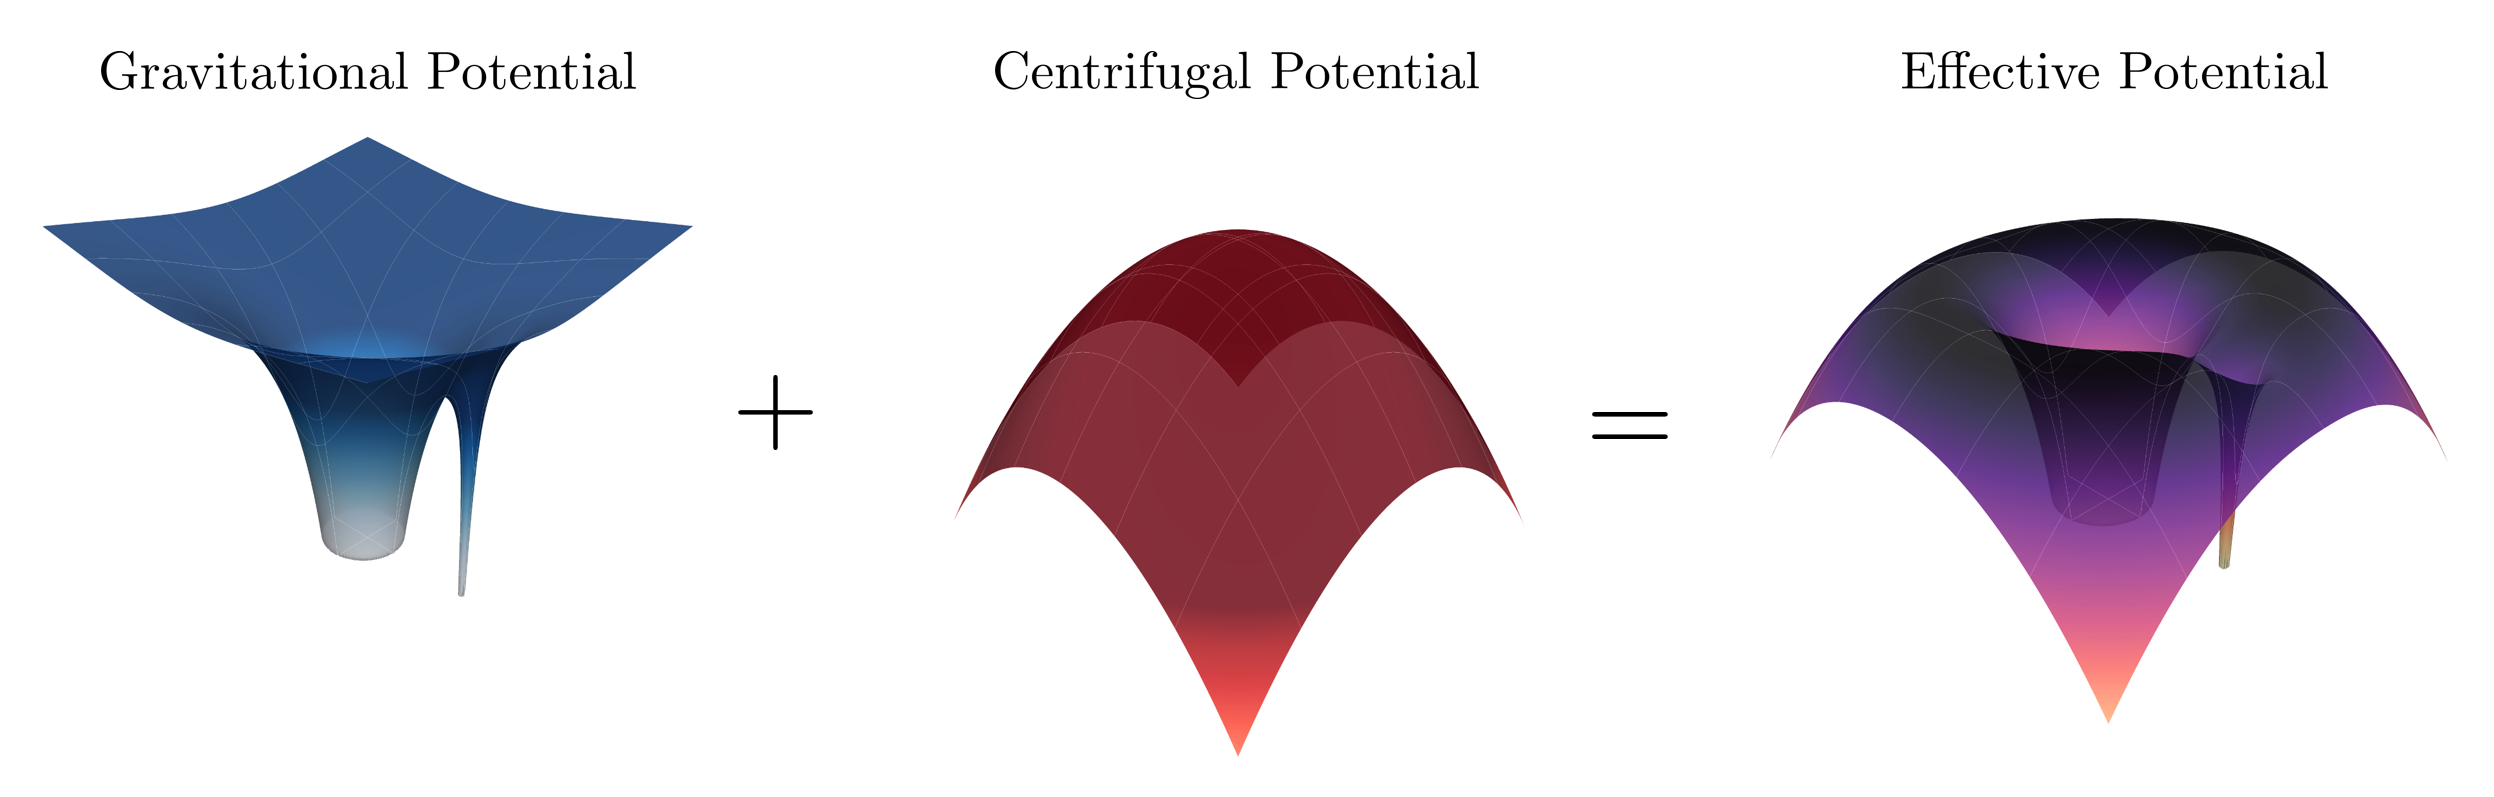
\includegraphics[width=\linewidth]{images/Potentials.png}
    \caption{Illustration of scalar potentials governing the CR3BP dynamics.}
    \label{fig:effective_potential}
\end{figure}

Since the system is closed, the total energy of the smallest body $m$ in the synodic frame is conserved. We identify the total energy as the sum of kinetic and potential energies. This quantity is the Hamiltonian of the system in \eqref{eq:cr3bp_acceleration}, written as
\begin{equation} \label{eq:hamiltonian_definition}
    H = \frac{1}{2}\|\boldsymbol{v}\|_2^2 + \tilde{U} = \frac{1}{2}\left(v_x^2 + v_y^2 +v_z^2\right) -\frac{1-\mu}{\rho_1} - \frac{\mu}{\rho_2} -\frac{1}{2}\left(x^2 + y^2\right).
\end{equation}
It is easy to show that the dynamics \eqref{eq:cr3bp_acceleration} can be rewritten in terms of the Hamiltonian as 
\begin{align*}
    \dot{\boldsymbol{r}} &= \nabla_{\boldsymbol{v}} H, \\
    \dot{\boldsymbol{v}} &= 
    \begin{pmatrix}
        0 & 2 & 0 \\
        -2 & 0 & 0 \\
        0 & 0 & 0
    \end{pmatrix}
    \nabla_{\boldsymbol{v}} H
    - \nabla_{\boldsymbol{r}} H,
\end{align*}
where the first term in the $\dot{\boldsymbol{v}}$ equation represents the Coriolis acceleration. We remark that this term can be eliminated by simply transforming to canonical coordinates; in these coordinates, the velocity $\boldsymbol{v}$ is replaced by canonical momentum $\boldsymbol{p}$, which, in the rotating frame, is given by $\boldsymbol{p} = (v_x -y, v_y+x, v_z)$. In $\boldsymbol{z} \coloneq(\boldsymbol{r}, \boldsymbol{p})$ coordinates, the system satisfies the Hamilton canonical equation
\begin{equation} \label{eq:hamilton_canonical_equation}
    \dot{\boldsymbol{z}} = \boldsymbol{J} \nabla H(\boldsymbol{z}), \qquad
    \boldsymbol{J} = \begin{pmatrix}
    0 & I \\
    - I & 0
    \end{pmatrix},
\end{equation}
where $\boldsymbol{J}$ is the canonical symplectic matrix. The CR3BP system is therefore Hamiltonian.


\clearpage

In the astrodynamics literature, the total energy of the CR3BP is often referred to in terms of the system's first integral of motion, the \emph{Jacobi integral} $C$, which can be written in terms of the Hamiltonian as
\begin{equation} \label{eq:jacobi_integral}
    C = -2H.
\end{equation}

The conservation of the Hamiltonian (and consequently the Jacobi integral) places strict topological bounds on the motion of the spacecraft. Because the kinetic energy must be a non-negative real value ($\frac{1}{2}\|\boldsymbol{v}\|_2^2 \ge 0$), the spacecraft is physically constrained to regions of space where its total energy is greater than or equal to the local effective potential:
\begin{equation*}
    C \leq 2\tilde{U}.
\end{equation*}
The boundaries of these allowed regions, defined by the condition where the kinetic energy drops exactly to zero ($C = 2\tilde{U}$), are known as the \emph{Zero Velocity Surfaces} (ZVS). In the planar case ($z=0$), these project as \emph{Zero Velocity Curves} (ZVC). The spatial volumes bounded by these surfaces are referred to as \emph{Hill's regions}. A spacecraft possessing a specific Hamiltonian cannot traverse the ZVS; it is strictly confined to the connected Hill's region in which it originated. These boundaries serve as hard reachability limits dictated by the combined gravitational and centrifugal landscapes, as visualized in \cref{fig:hills_regions}.

\begin{figure}[htbp]
    \centering

    \begin{subfigure}{0.4\textwidth}
        \centering
        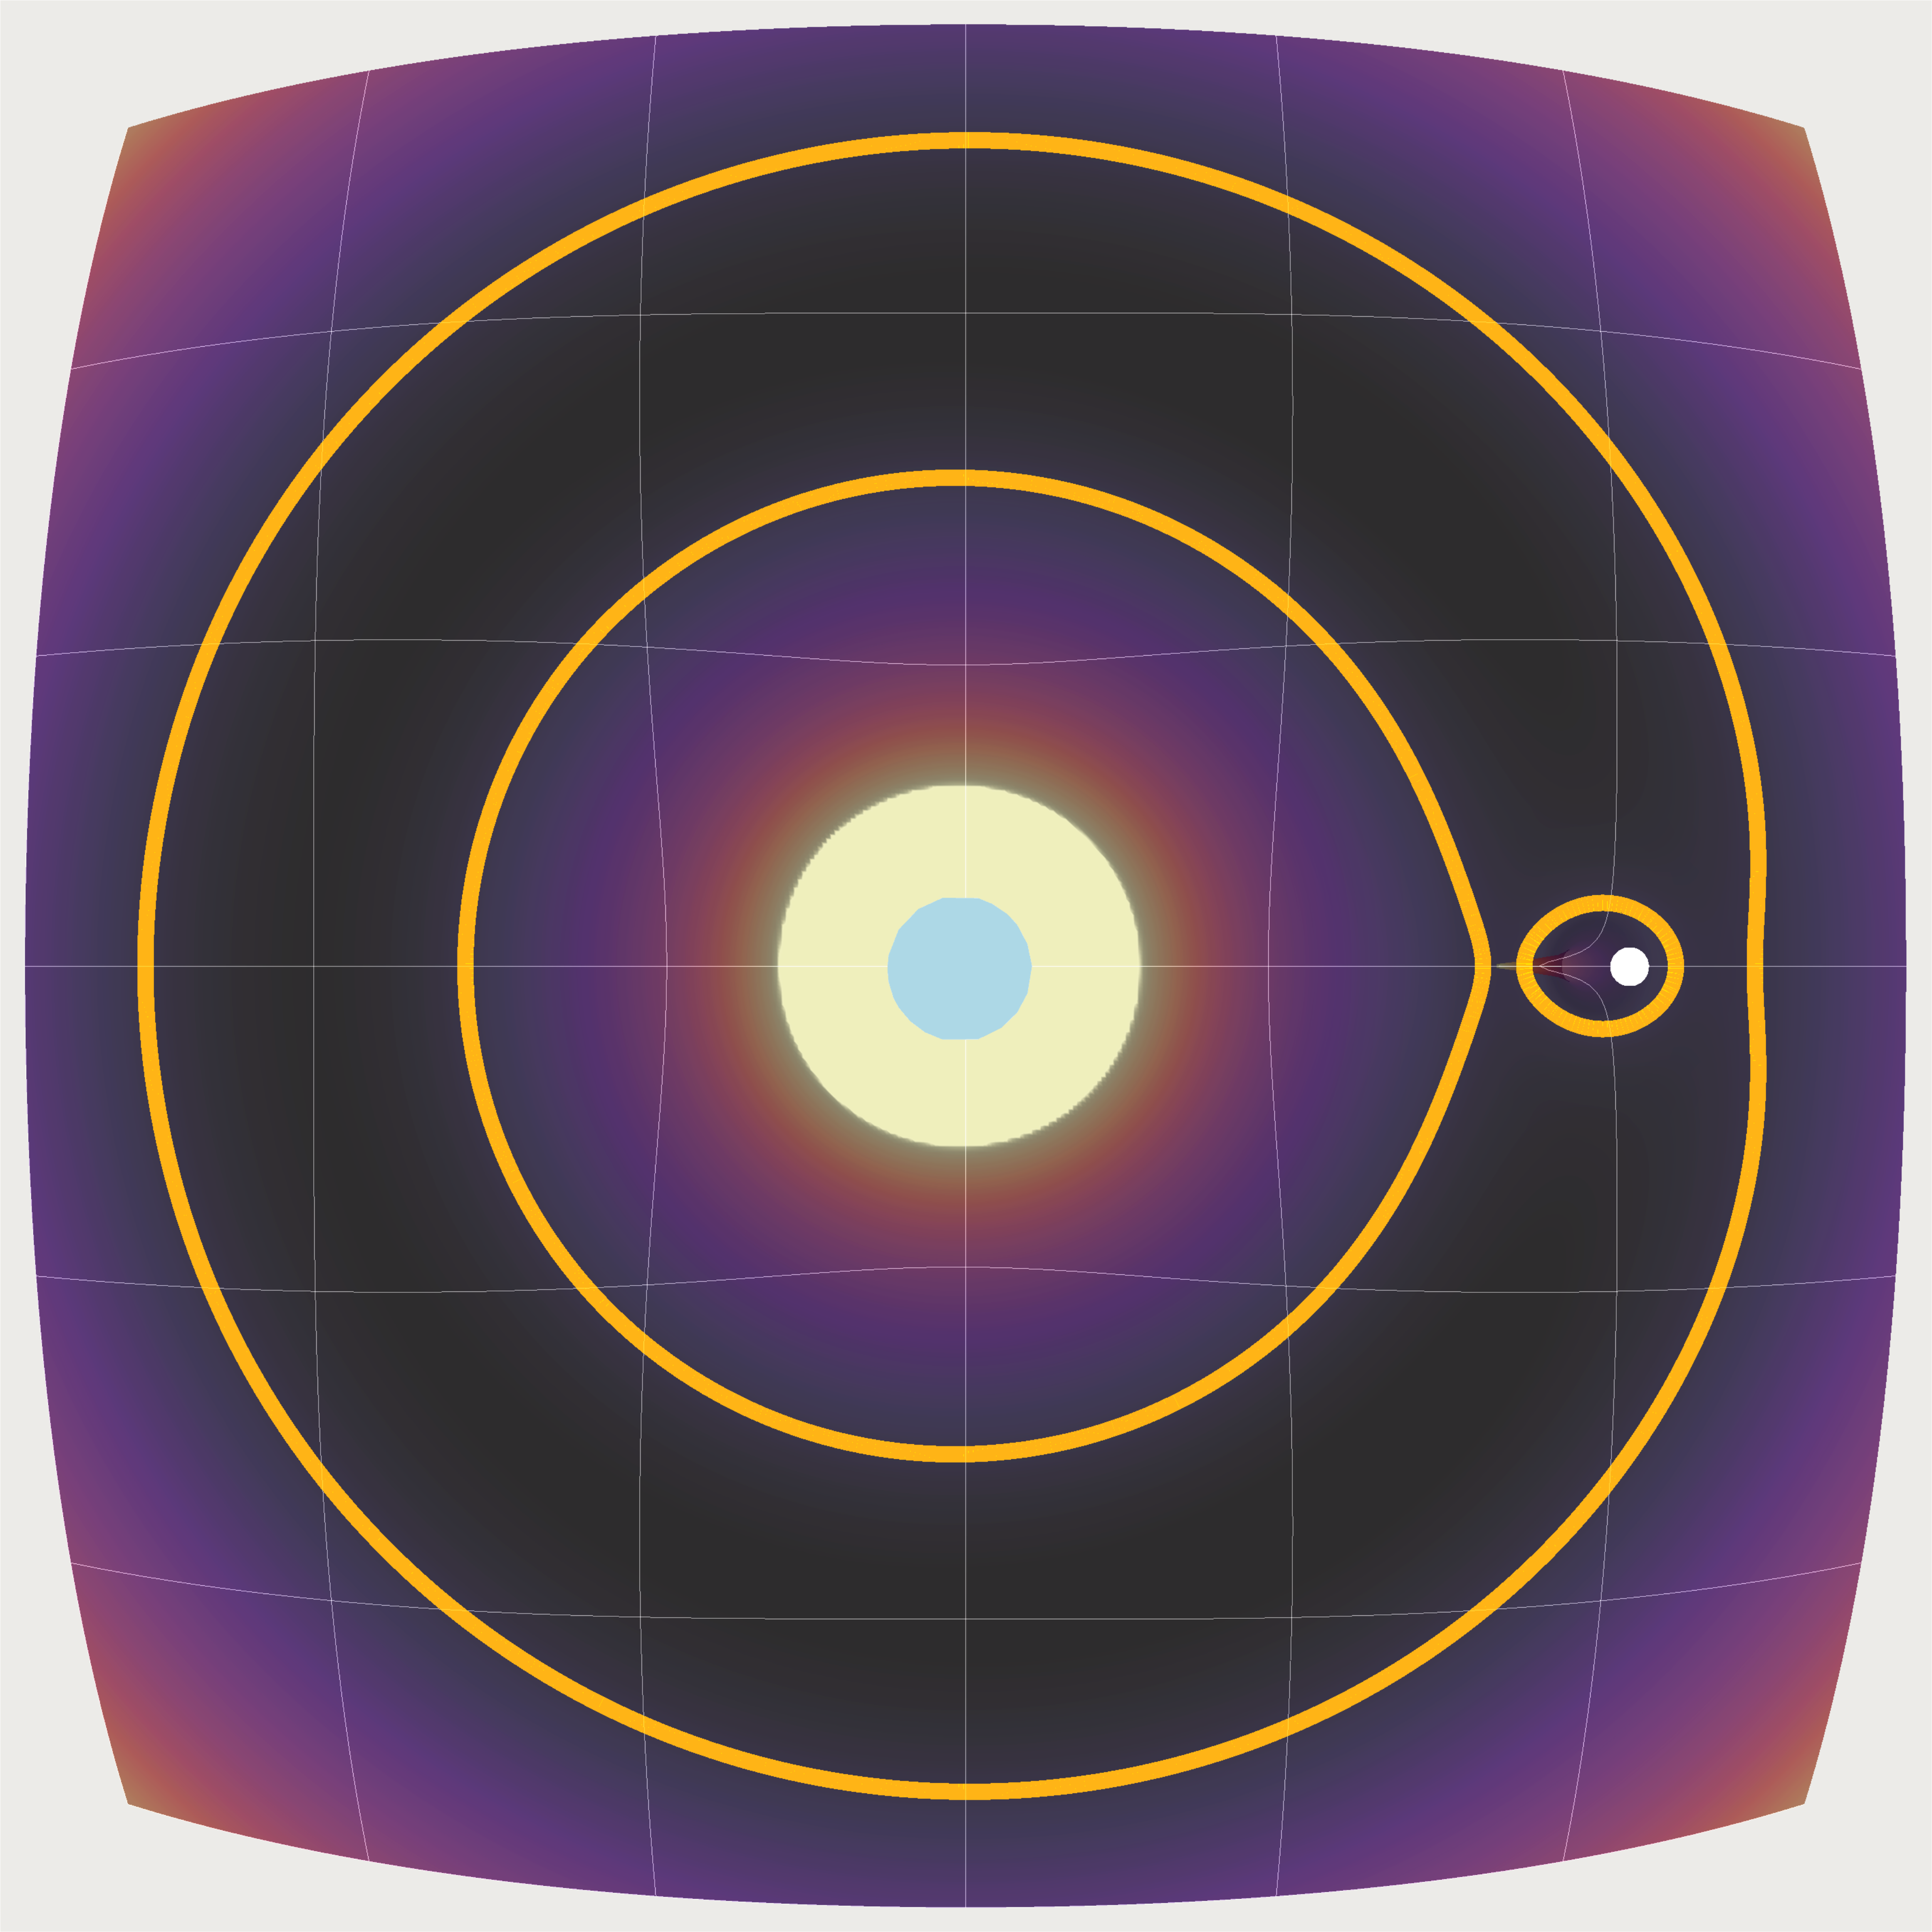
\includegraphics[width=\linewidth]{images/hill_curve_3.20.png}
        \caption{$C \in (C_1, C_2)$}
        \label{fig:hills_regions_c1c2}
    \end{subfigure}
    \hspace{1.5em}
    \begin{subfigure}{0.4\textwidth}
        \centering
        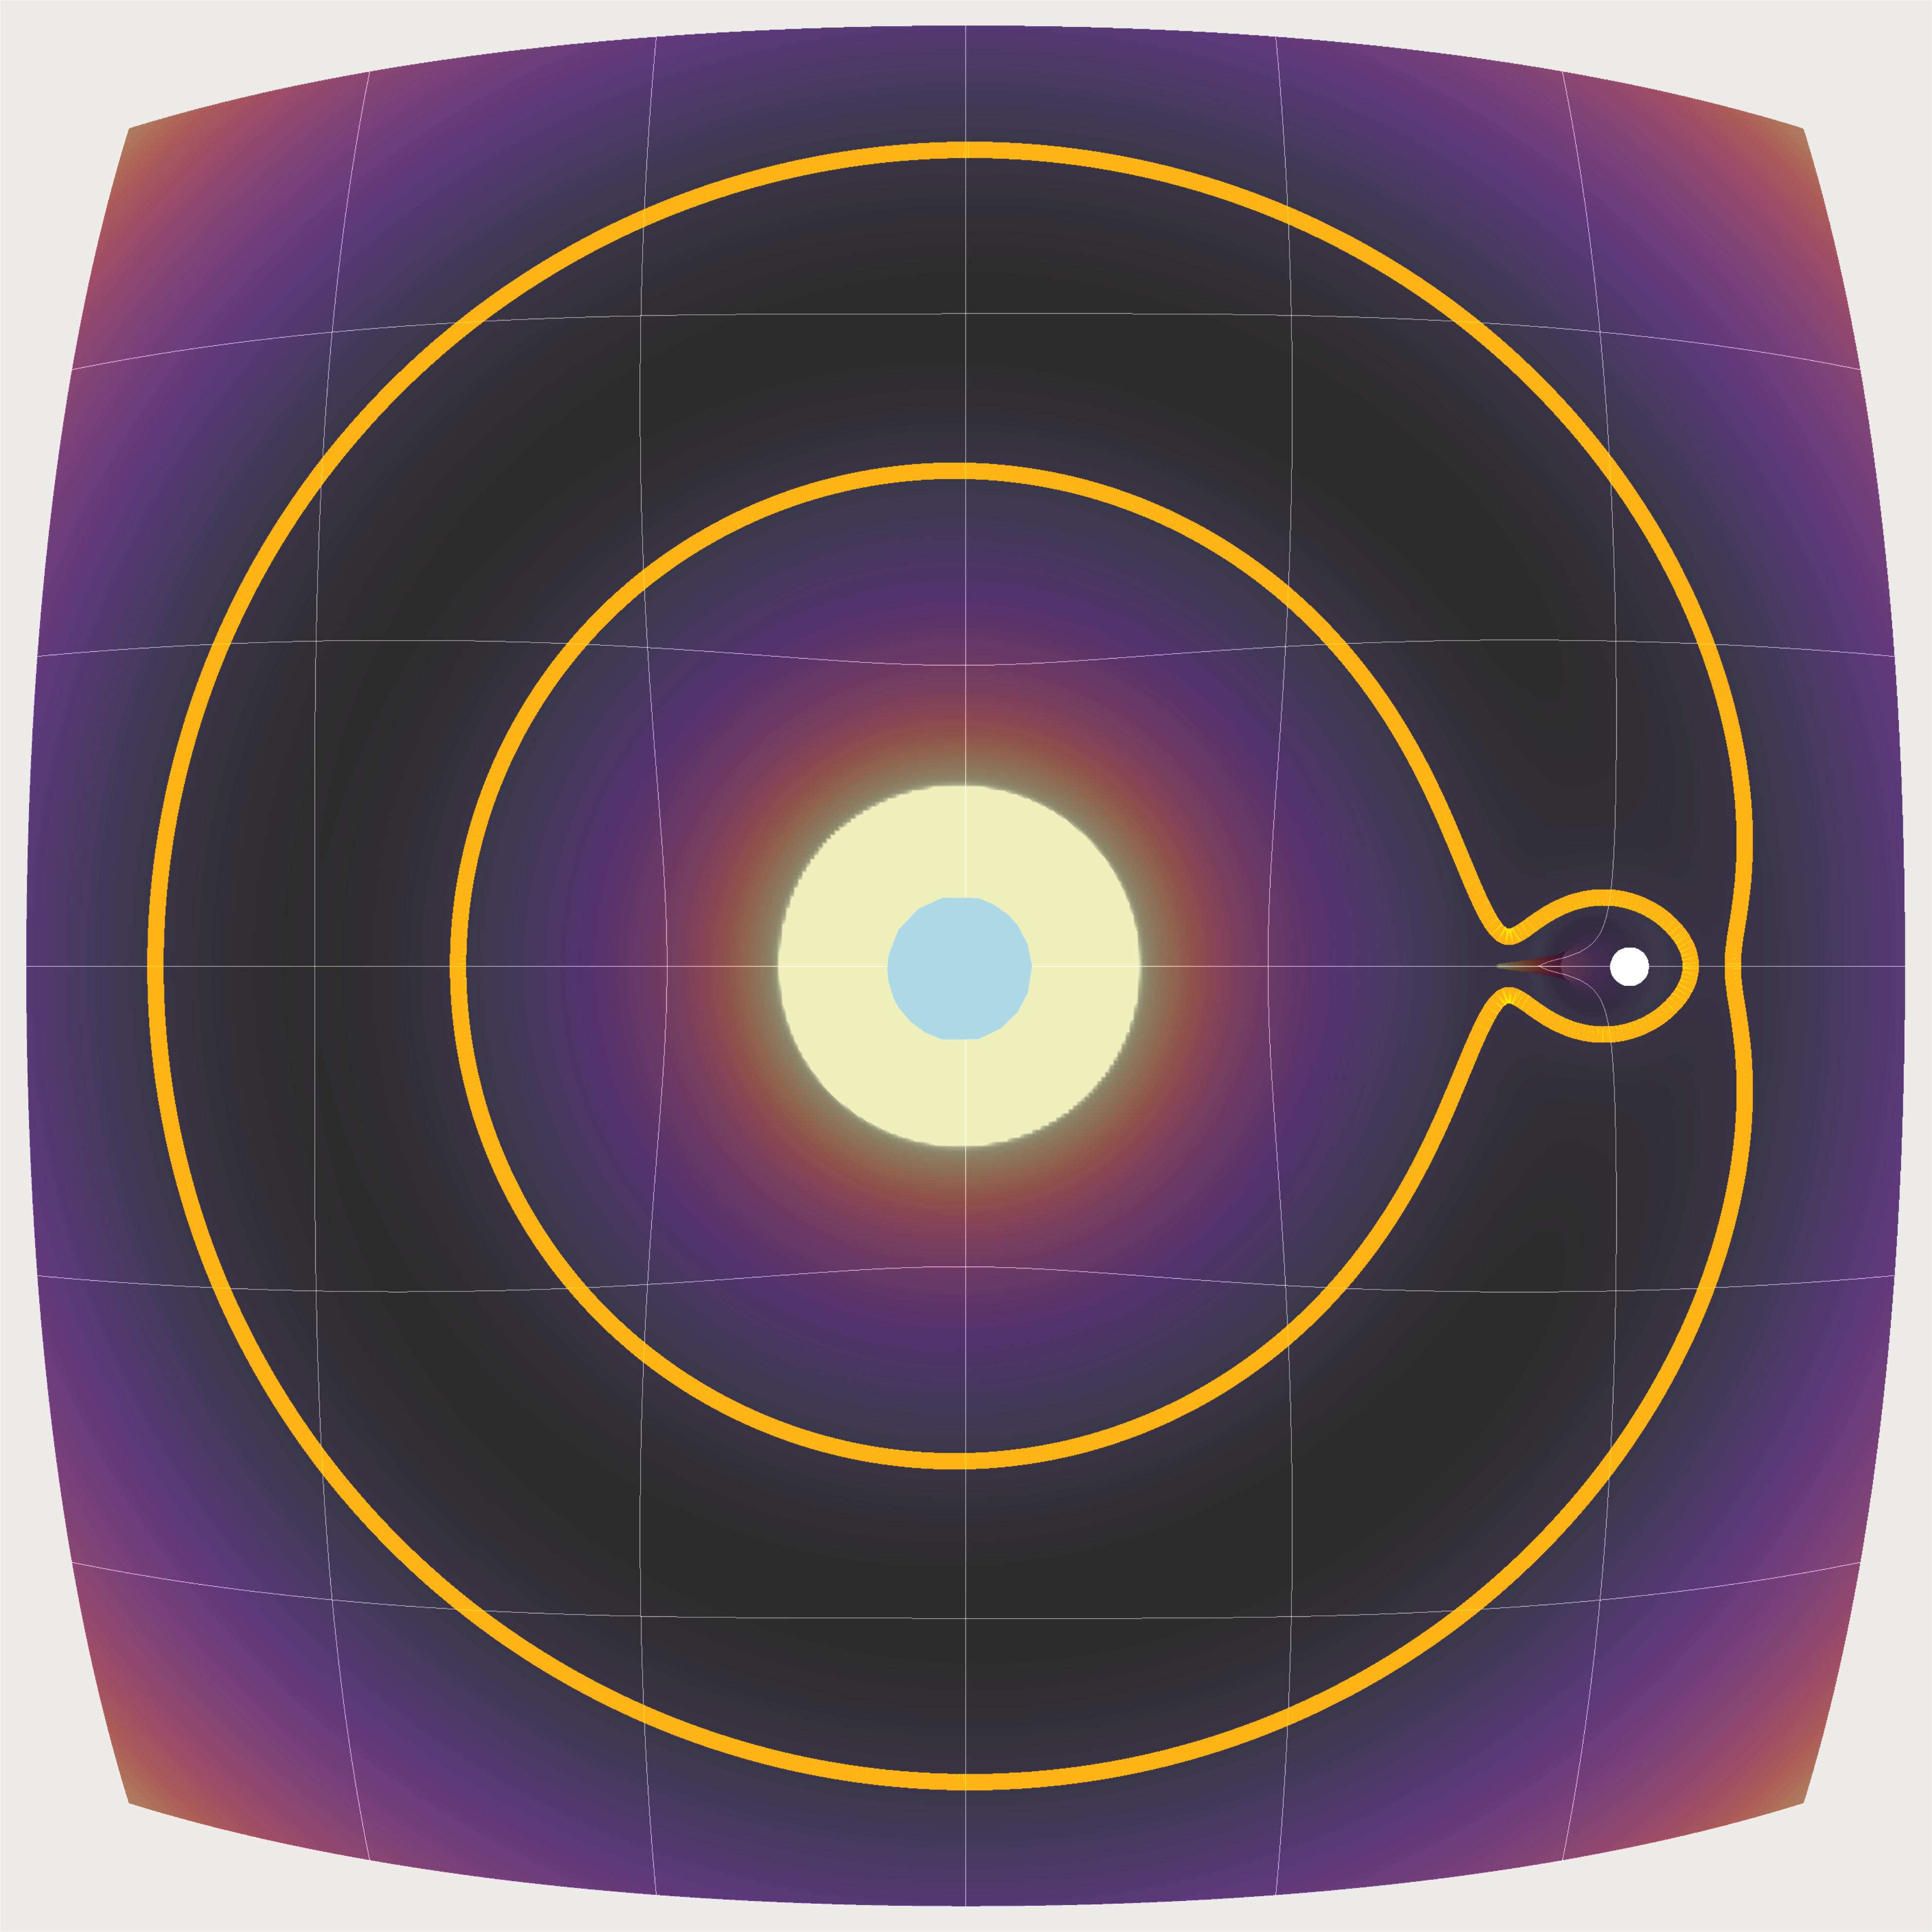
\includegraphics[width=\linewidth]{images/hill_curve_3.18.png}
        \caption{$C \in (C_2, C_3)$}
        \label{fig:hills_regions_c2c3}
    \end{subfigure}

    \vspace{0.5em}

    \begin{subfigure}{0.4\textwidth}
        \centering
        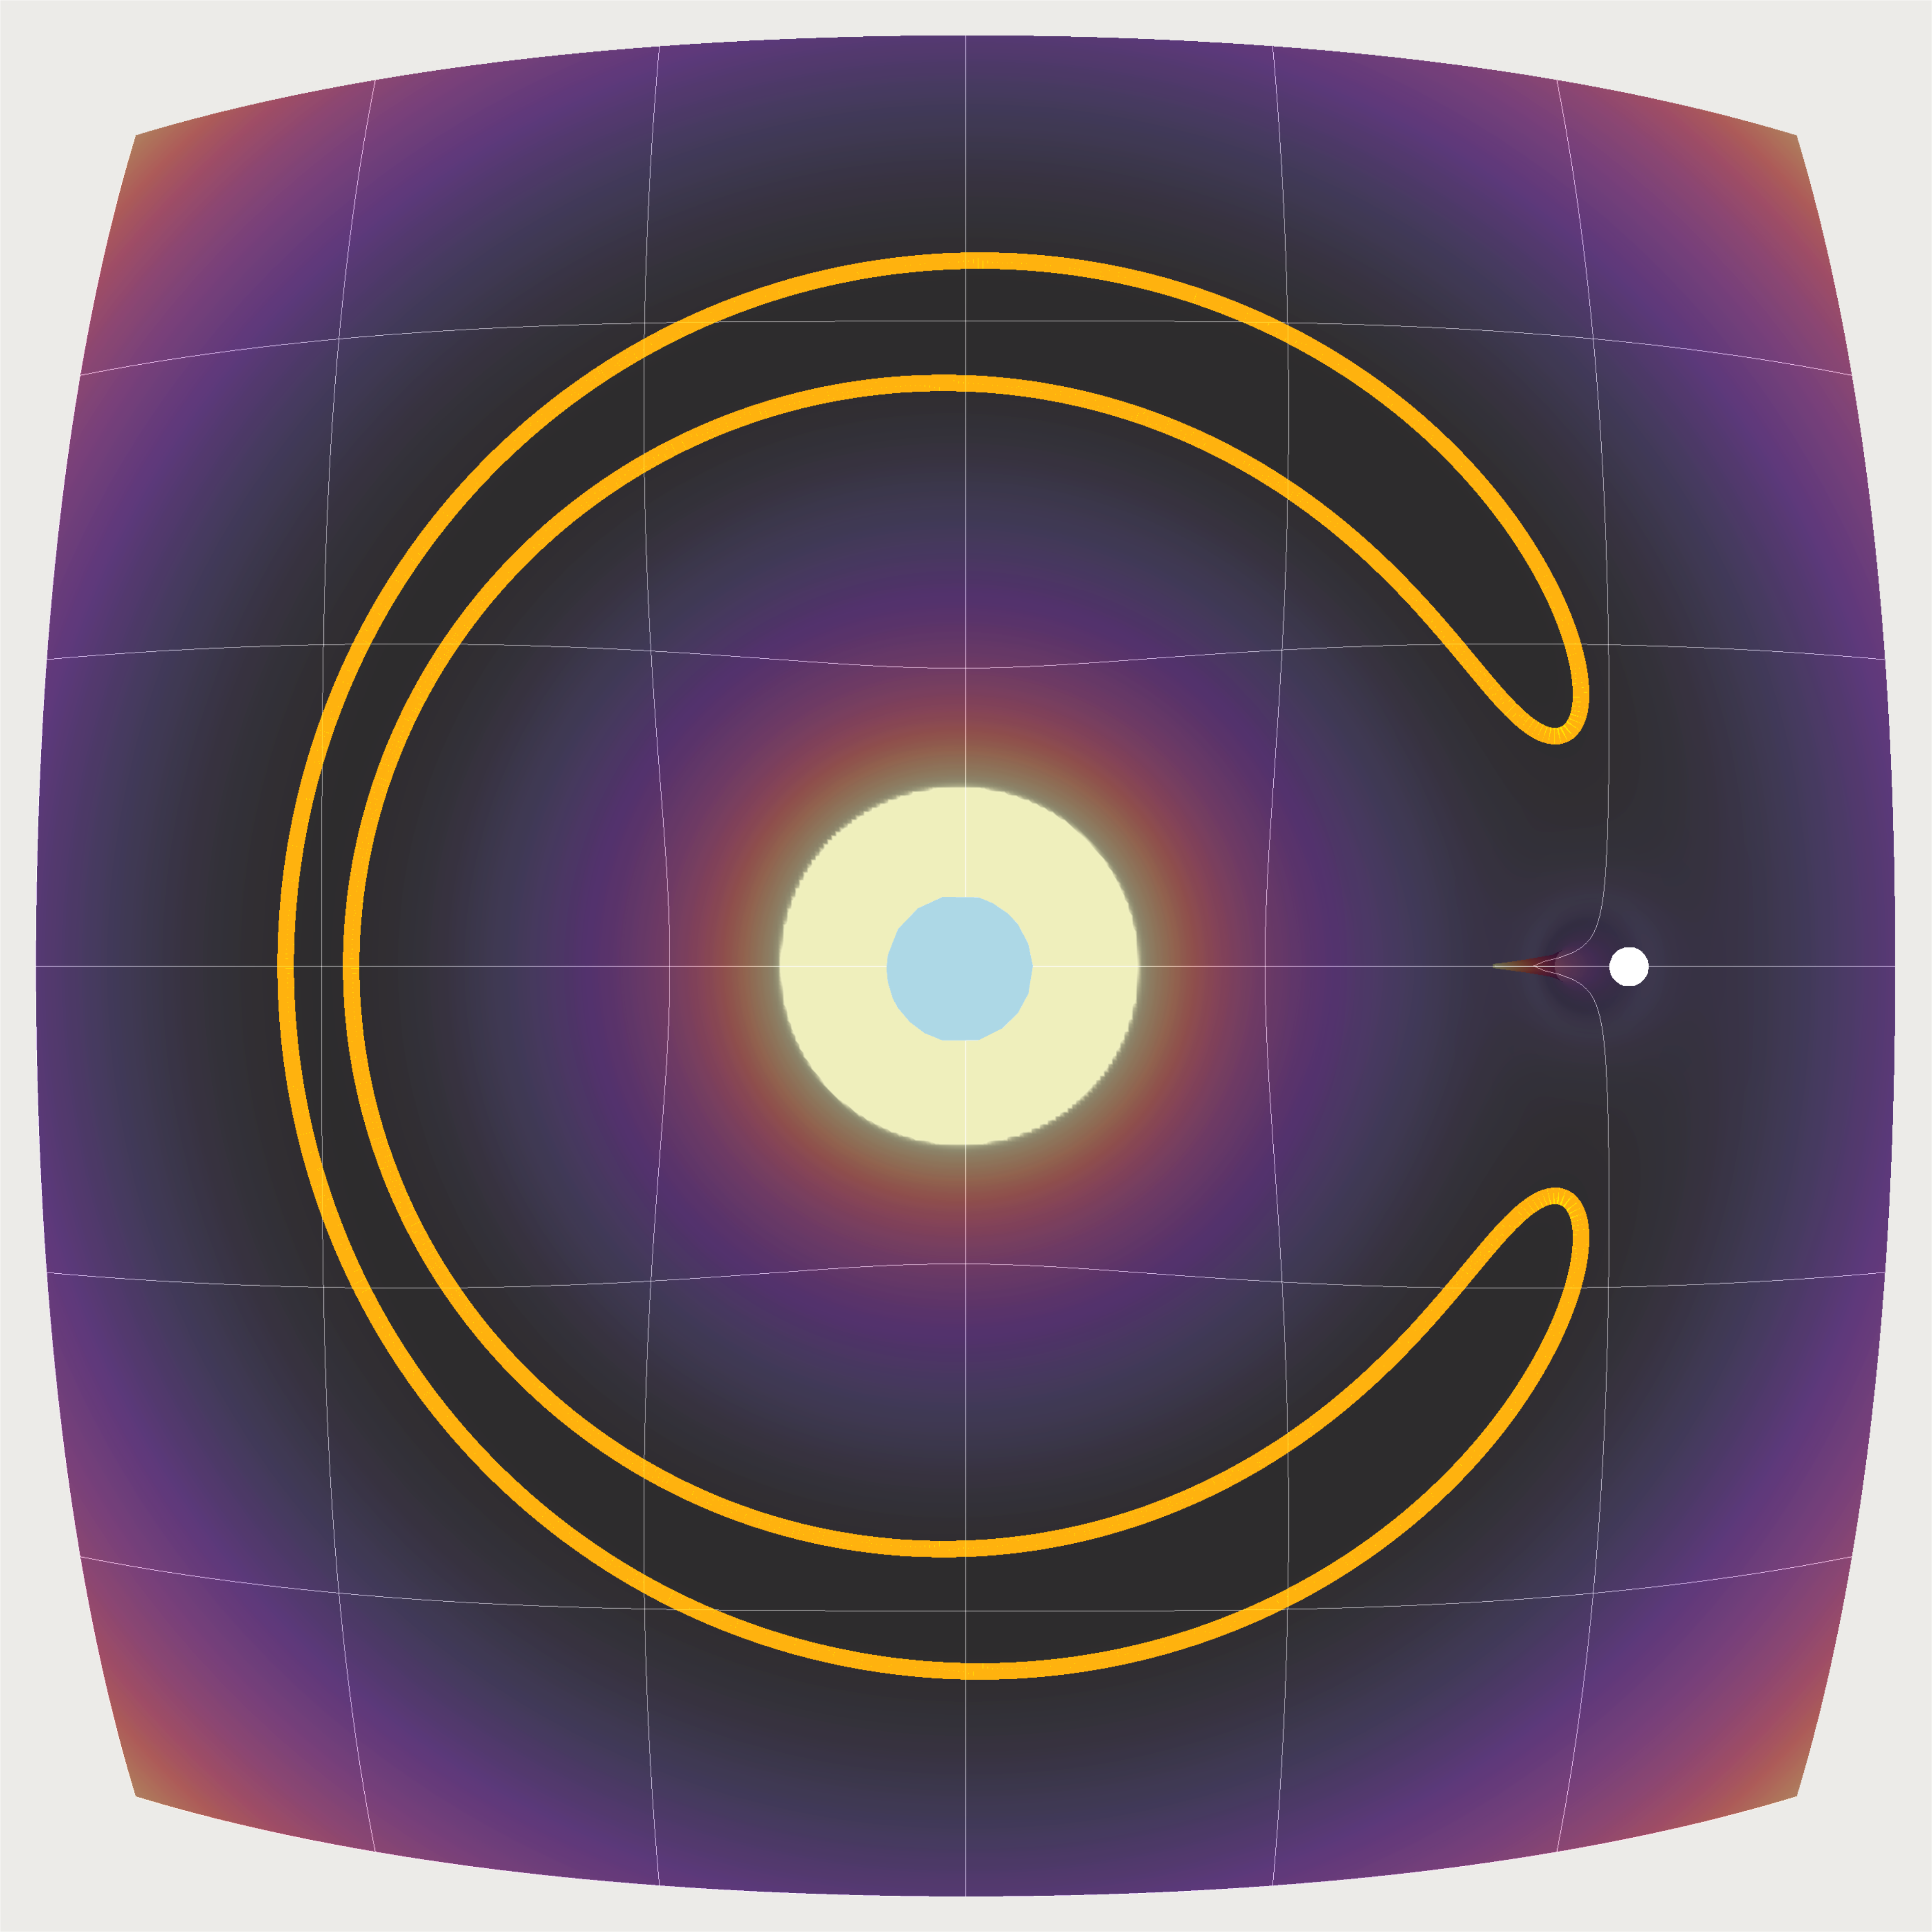
\includegraphics[width=\linewidth]{images/hill_curve_3.02.png}
        \caption{$C \in (C_3, C_4)$}
        \label{fig:hills_regions_c3c4}
    \end{subfigure}
    \hspace{1.5em}
    \begin{subfigure}{0.4\textwidth}
        \centering
        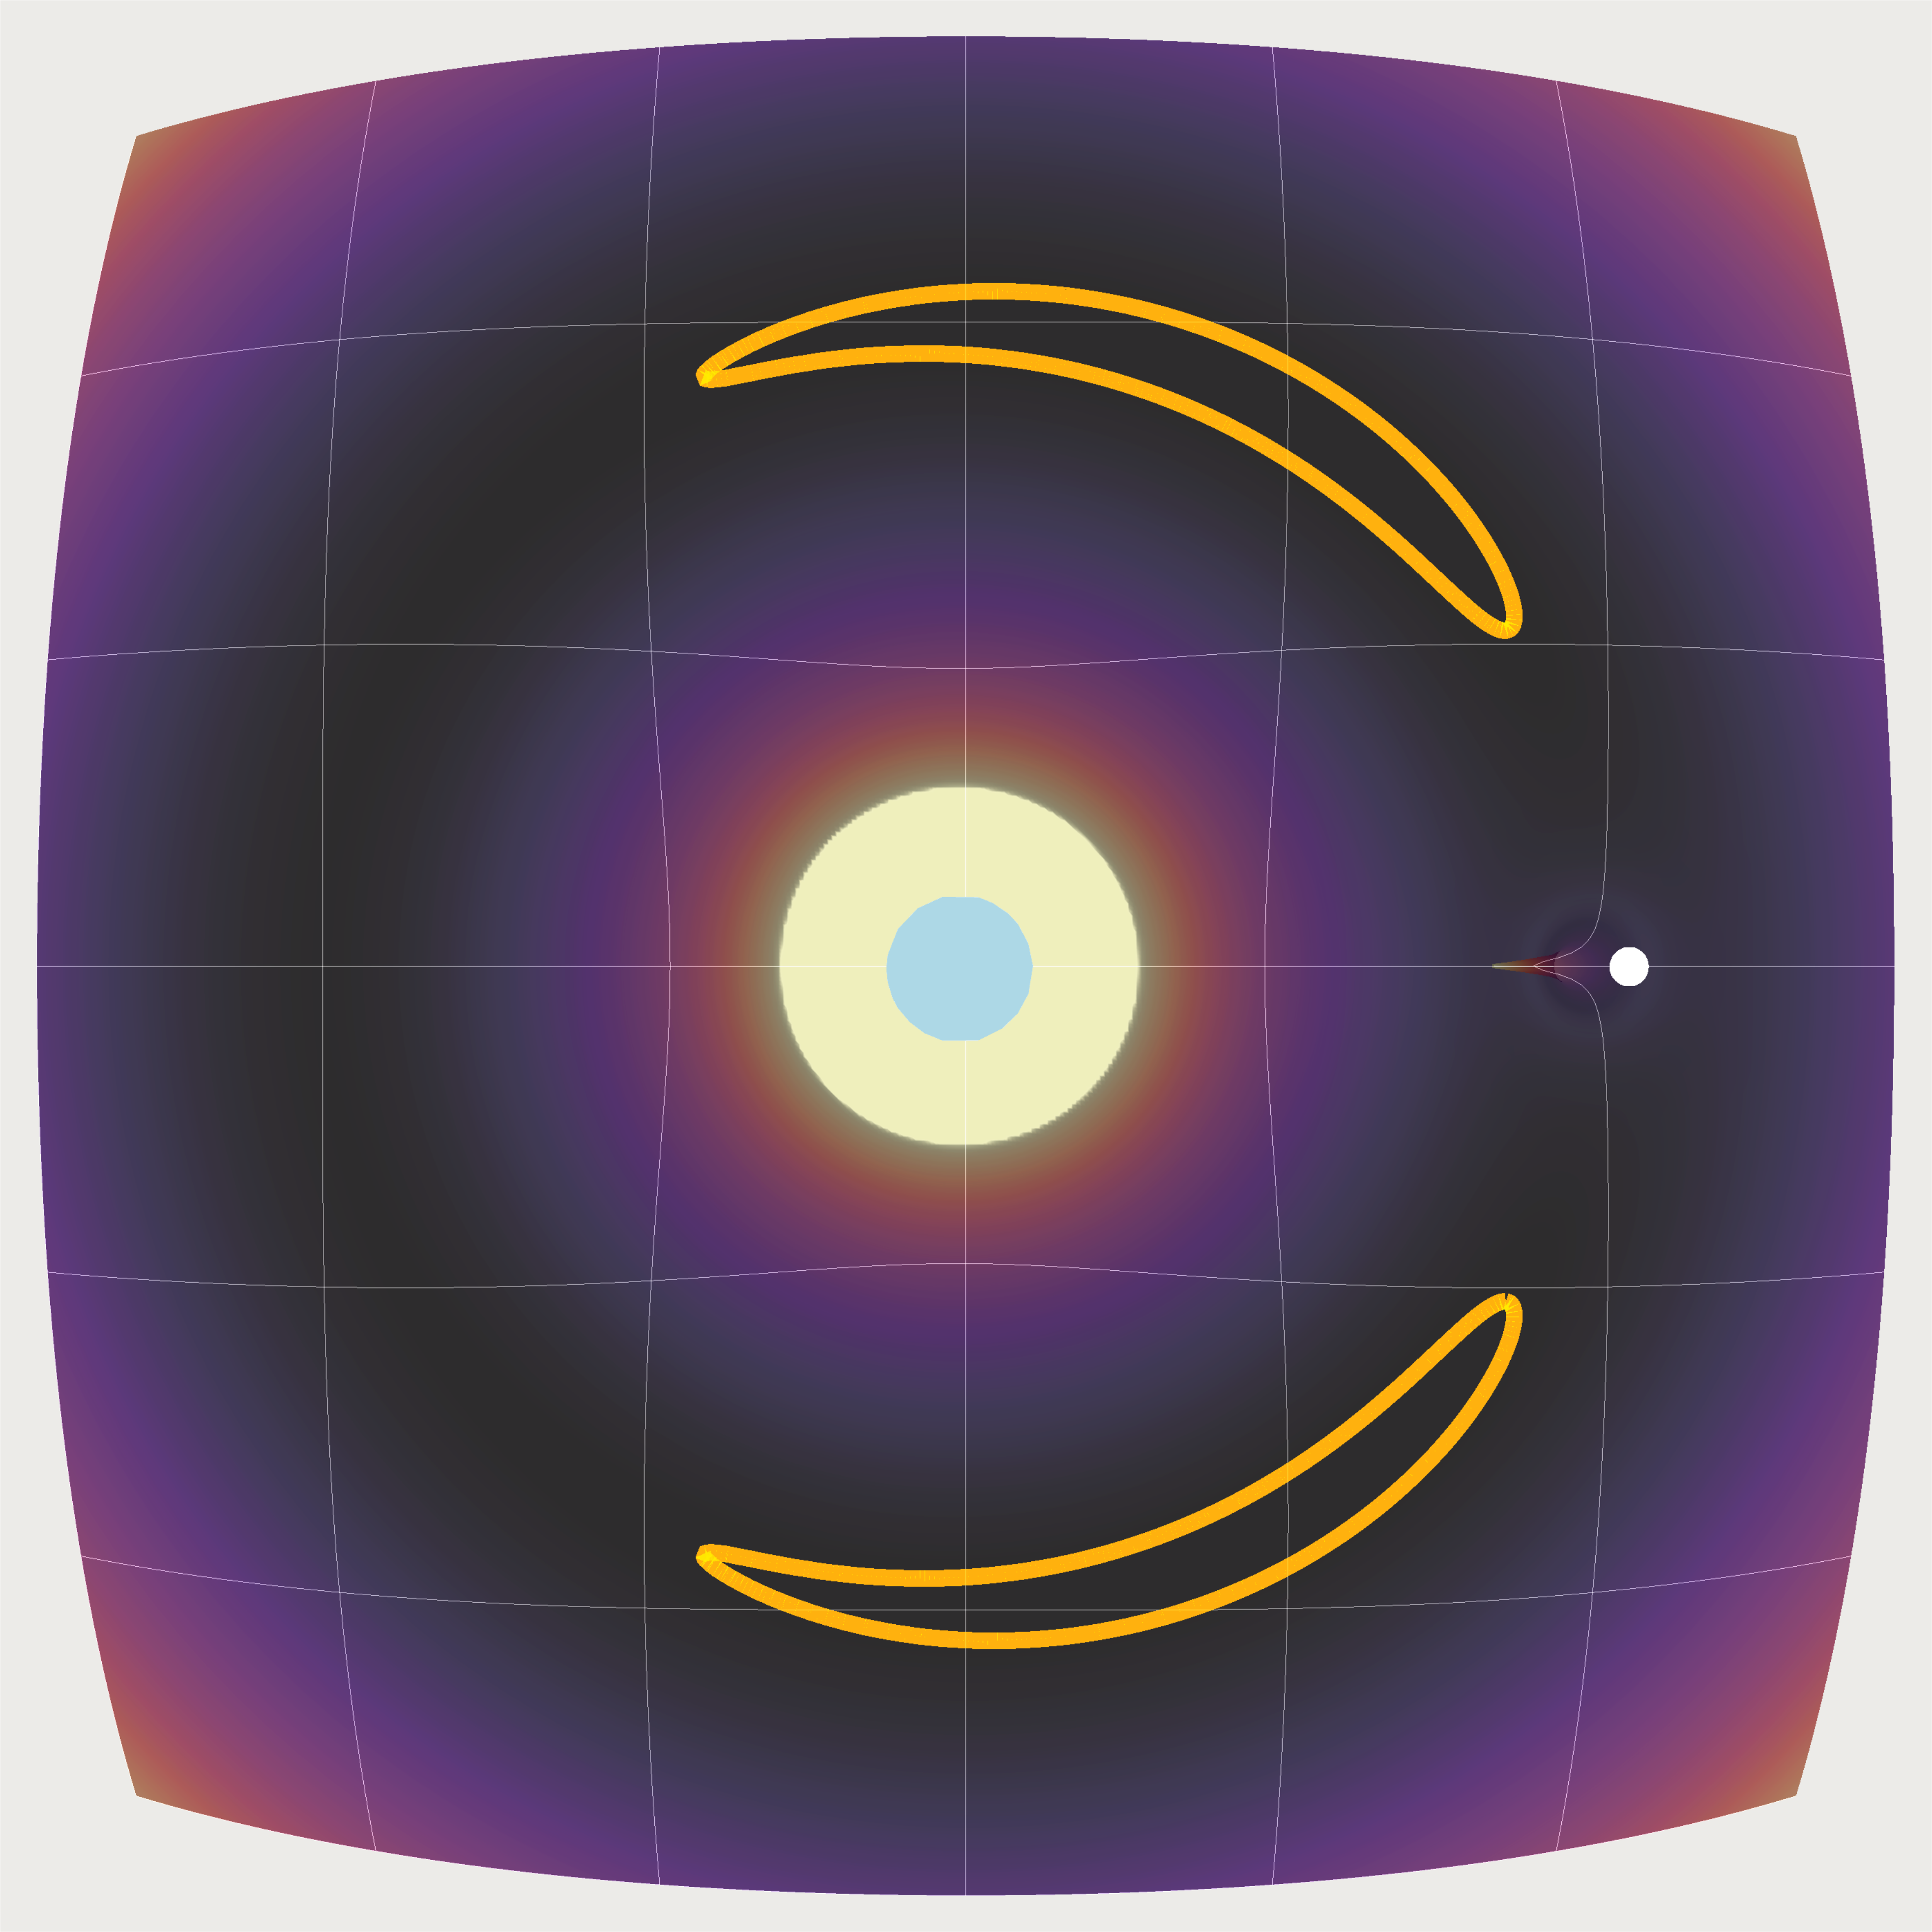
\includegraphics[width=\linewidth]{images/hill_curve_3.00.png}
        \caption{$C \in (C_4, C_5)$}
        \label{fig:hills_regions_c4c5}
    \end{subfigure}

    \caption{Hill's regions across Jacobi integral ranges.}
    \label{fig:hills_regions}
\end{figure}

\clearpage

\begin{figure}[htbp]
    \centering
    \begin{tikzpicture}
        \begin{axis}[
            axis equal image,
            hide axis,
            width=8cm, 
            height=9cm,
            clip=false,
            axis lines=middle,
            ticks=none
        ]
    
        % Masses m1 and m2
        \addplot[mark=*, mark size=6pt, only marks, color=brown!90!red] coordinates {(-0.13, 0)}; 
        \node at (axis cs:-0.13, 0.06) {$m_1$}; 
        \node at (axis cs:-0.15, -0.07) {$(-\mu, 0, 0)$}; 
        \addplot[mark=*, mark size=4pt, only marks, color=brown!90!red] coordinates {(0.41, 0)}; 
        \node at (axis cs:0.41, 0.05) {$m_2$}; 
        \node at (axis cs:0.46, -0.175) {$(1 - \mu, 0, 0)$}; 
        \draw[] (axis cs:0.46, -0.15) -- (axis cs:0.42, -0.03);
    
        % Adding nodes L4 and L5
        \addplot[mark=x, mark size=3pt, thick, only marks, color=blue] coordinates {(0.14, 0.468)}; 
        \node at (axis cs:0.2, 0.468) {$\mathcal{L}_4$};
        
        \addplot[mark=x, mark size=3pt, thick, only marks, color=blue] coordinates {(0.14, -0.468)}; 
        \node at (axis cs:0.2, -0.468) {$\mathcal{L}_5$};
    
        % Adding nodes L1,L2 and L3
        \addplot[mark=x, mark size=3pt, thick, only marks, color=blue] coordinates {(0.27, 0)}; 
        \node at (axis cs:0.27, 0.05) {$\mathcal{L}_1$};
        
        \addplot[mark=x, mark size=3pt, thick, only marks, color=blue] coordinates {(0.55, 0)}; 
        \node at (axis cs:0.55, 0.05) {$\mathcal{L}_2$};
    
        \addplot[mark=x, mark size=3pt, thick, only marks, color=blue] coordinates {(-0.5, 0)}; 
        \node at (axis cs:-0.5, 0.05) {$\mathcal{L}_3$};
        
        % Point P
        \addplot[mark=*, mark size=1.5pt, only marks, color=black] coordinates {(0.25, 0.275)}; 
        \node at (axis cs:0.25, 0.315) {$P$}; 
        \node at (axis cs:0.25, 0.235) {$(x, y, z)$}; 
    
        % Axes
        \draw[->, >=stealth, thick] (-0.55, 0) -- (0.8, 0) node[ below] {$x$}; 
        \draw[->, >=stealth, thick] (0, -0.5) -- (0, 0.6) node[left] {$y$}; 
        %\draw[->, >=stealth, thick] ($(0.07*1.4142, 0.07*1.4142)$) -- ($(-0.07*1.4142, -0.07*1.4142)$) node[below right] {$z$}; 
    
        % Setting axis limits
        \path (axis cs:-0.125,-0.1) rectangle (axis cs:0.6,0.5); 
    
        \end{axis}
    \end{tikzpicture}
    \caption{Caption}
    \label{fig:placeholder}
\end{figure}

